\documentclass[a4paper]{article}

\usepackage[pages=all, color=black, position={current page.south}, placement=bottom, scale=1, opacity=1, vshift=5mm]{background}
\usepackage[margin=1in]{geometry} % full-width

% AMS Packages
\usepackage{amsmath}
\usepackage{amsthm}
\usepackage{amssymb}
\usepackage[hidelinks]{hyperref}
% Unicode
\usepackage[utf8]{inputenc}
\usepackage{hyperref}
\hypersetup{
	unicode,
%	colorlinks,
%	breaklinks,
%	urlcolor=cyan, 
%	linkcolor=blue, 
	pdfauthor={Author One, Author Two, Author Three},
	pdftitle={A simple article template},
	pdfsubject={A simple article template},
	pdfkeywords={article, template, simple},
	pdfproducer={LaTeX},
	pdfcreator={pdflatex}
}

% Vietnamese
%\usepackage{vntex}

% Natbib
\usepackage[sort&compress,numbers,square]{natbib}
\bibliographystyle{mplainnat}

% Theorem, Lemma, etc
\theoremstyle{plain}
\newtheorem{theorem}{Theorem}
\newtheorem{corollary}[theorem]{Corollary}
\newtheorem{lemma}[theorem]{Lemma}
\newtheorem{claim}{Claim}[theorem]
\newtheorem{axiom}[theorem]{Axiom}
\newtheorem{conjecture}[theorem]{Conjecture}
\newtheorem{fact}[theorem]{Fact}
\newtheorem{hypothesis}[theorem]{Hypothesis}
\newtheorem{assumption}[theorem]{Assumption}
\newtheorem{proposition}[theorem]{Proposition}
\newtheorem{criterion}[theorem]{Criterion}
\theoremstyle{definition}
\newtheorem{definition}[theorem]{Definition}
\newtheorem{example}[theorem]{Example}
\newtheorem{remark}[theorem]{Remark}
\newtheorem{problem}[theorem]{Problem}
\newtheorem{principle}[theorem]{Principle}

\usepackage{graphicx, color}
\graphicspath{{fig/}}

%\usepackage[linesnumbered,ruled,vlined,commentsnumbered]{algorithm2e} % use algorithm2e for typesetting algorithms
\usepackage{algorithm, algpseudocode} % use algorithm and algorithmicx for typesetting algorithms
\usepackage{mathrsfs} % for \mathscr command

\usepackage{lipsum}

% Author info
\title{\textbf{\Huge Face Identification}
\vspace{10mm}}
\vspace{10mm}
\author{\Large Dhyey Findoriya \and \Large Akshat Patidar\and \Large Nisarg Vaghela\and \Large  Manas Chechani\and \Large Ankit Raj}

\date{
\vspace{10mm}
	\textbf{Course Project}:   Pattern Recognition and Machine Learning-CSL2050\\ %
 \vspace{5mm} Spring Semester-2024: IIT Jodhpur%
%	\today
}

\begin{document}
	\maketitle
	\vspace{25mm}
	

	\tableofcontents
 

\vspace{50mm}
	\section{\LARGE Introduction}
	\label{sec:intro}
	
    \Large
         In our increasingly digital world, the accurate identification of faces holds significant importance across diverse fields. This project focuses on the task of face identification, wherein a given face image is classified into one of several predefined classes. 
 \newline           We employ three distinct feature extraction techniques – Local Binary Patterns (LBP), Histogram of Oriented Gradients (HoG), and Convolutional Neural Networks (CNNs) ,Linear Discriminant Ananlysis (LDA) and Principal Component Ananlysis (PCA)
– to capture unique facial characteristics.

Our aim is to compare the effectiveness of these techniques in identifying faces using the Labeled Faces in the Wild (LFW) dataset sourced from Kaggle. This dataset, provides a comprehensive collection of labeled face images suitable for training and evaluation.

Throughout this report, we detail the implementation of each feature extraction method, the experimental setup, and the comparative analysis of their performance in face identification. This project serves as a valuable exploration of multimodal feature analysis in the context of facial recognition, offering insights into its potential applications and limitations.
	

	\newpage
	
	
	\section{Approaches Tried}
	\label{sec:app}
	We have tried five approaches for our problem statement in order to get better result. The details and findings of all are cited below.

        \subsection{Local Binary Pattern Extraction}
	Local Binary Pattern (LBP) extraction is a technique used in image processing and computer vision for texture analysis and feature extraction. It's particularly popular in tasks like facial recognition, texture classification, and object detection. LBP is robust to monotonic gray-scale changes and relatively invariant to changes in illumination, making it useful in real-world scenarios where lighting conditions may vary.\bigskip

    The implementation part is explained:-
    \subsubsection{Defining extract\_lbp\_features}
    The extract\_lbp\_features function takes images as arguments and converts each RGB image in the input list to grayscale using rgb2gray.
    And also computes the Local Binary Pattern (LBP) using local\_binary\_pattern with parameters P=8, R=1, and method='uniform'.
    And then calculates the histogram of the LBP values and appends it to the lbp\_features list. And finally Returns the LBP features as a numpy array.

    \subsubsection{Applying the defined function}
    Extracted LBP features from the filtered training images and the filtered test images by passing (X\_train\_filtered) and (X\_test\_filtered) respectively as arguments in the function.

    \subsubsection{Saving the extracted features}
    Saves the LBP features of the training dataset to a numpy file named lbp\_train\_features.npy and the LBP features of the test dataset to a numpy file named lbp\_test\_features.npy.

    \subsubsection{Classification}
    Finally we trained and evaluated multiple classifiers using the classifiers Support Vector Machine, Random Forest, K-Nearest Neighbors, and Gradient Boosting. The accuracy of each classifier is calculated and printed out.

        \subsection{Histogram of Oriented Gradient}

Histogram of Oriented Gradients (HOG) is a feature descriptor used in image processing and computer vision for object detection and recognition tasks. It is particularly effective in detecting objects with well-defined edges and textures, such as human faces and pedestrian silhouettes. 

Our implementation process is explained in the following way:-
        \subsubsection{Defining extract\_hog\_features}
The function takes images as arguments and computes HOG features with specified parameters for each image in the input list. And returns the HOG features as a numpy array.

        \subsubsection{Applying the defined function}
Calculated HOG features for the filtered training images and for the filtered test images by passing (X\_train\_filtered) and (X\_test\_filtered) respectively.

        \subsubsection{Saving the extracted features}
Saving the HOG features of the training dataset to a numpy file named hog\_train\_features.npy and of the test dataset to a numpy file named hog\_test\_features.npy.

        \subsubsection{Classification}
Finally we trained and evaluated multiple classifiers using the classifiers Support Vector Machine, Random Forest, K-Nearest Neighbors, and Gradient Boosting. The accuracy of each classifier is calculated and printed out.
        
        \subsection{Convolutional Neural Network}
	
\setlength {\parindent}{10pt} Type of deep learning model designed for tasks like image recognition. It uses layers that learn to identify patterns in images, like edges and textures, and progressively combine them to recognize more complex features.\bigskip

And our approach to implement it in our project is cited below:

        \subsubsection{Extract CNN Feature}
        The extract\_cnn\_features function utilizes the VGG16 pre\-trained model to extract CNN features from a collection of images. Specifically, it captures the features from the 'block5\_conv2' layer of the VGG16 model. The function preprocesses each image, feeds it through the model, and flattens the extracted features. And the resulting CNN features are returned as a numpy array.

        \subsubsection{Applying Function on Filtered Dataset}
        The extract\_cnn\_features function is applied to the filtered training and test image datasets (X\_train\_filtered and X\_test\_filtered) to extract CNN features using the VGG16 model. The resulting CNN-transformed features are stored in cnn\_train\_features and cnn\_test\_features, respectively.

        \subsubsection{Saving the Extracted Features}
        The extracted CNN features from the filtered training and test image datasets (cnn\_train\_features and cnn\_test\_features) are saved as NPY files named cnn\_train\_features.npy and cnn\_test\_features.npy, respectively.

        \subsubsection{Training and Evaluation Classifier}
        Finally we trained and evaluated multiple classifiers using CNN features (cnn\_train\_features and cnn\_test\_features) extracted from filtered image datasets (X\_train\_filtered and X\_test\_filtered). The classifiers used are Support Vector Machine (SVM), Random Forest, K-Nearest Neighbors (KNN), and Gradient Boosting. The accuracy of each classifier is calculated and printed out.

        \subsection{Principal Component Analysis}
        PCA is mainly used as the dimensionality reduction technique in various AI applications such as computer vision, image compression, etc.\bigskip

	This is the 4th approach we worked upon and it is implemented in the following way.

        \subsubsection{Extract PCA Feature}
	The extract\_pca\_feautures function takes a collection of images and an optional number of principal components as input. It reshapes the images into a 2D array, and applies PCA to reduce the dimensionality, and returns the PCA transformed features.
        
        \subsubsection{Plotting Cummulative Variance Ratio}
        The plot\_cumulative\_variance\_ratio function calculates and plots the cumulative explained variance ratio against the number of principal components for a given collection of images. It determines the optimal number of components required to explain variance ranging from 10\% to 95\%, with a step size of 0.05. The function visualizes this relationship using matplotlib library.

        \subsubsection{Finding Optimal n\_component}
        The find\_optimal\_n\_components\ function calculates the optimal number of principal components needed to explain at least 85\% of the variance in a given collection of images. It uses PCA to determine this and returns the optimal number of components.

        \subsubsection{Transformation of Dataset}
        The extract\_pca\_features function is used to transform the filtered training and test image datasets (X\_train\_filtered and X\_test\_filtered) into PCA features with 120 principal components each. The resulting PCA-transformed features are stored in pca\_train\_features and pca\_test\_features, respectively.

        \subsubsection{Saving the Transformed Dataset}
        The PCA-transformed features of the filtered training and test image datasets (pca\_train\_features and pca\_test\_features) are saved as NPY files named pca\_train\_features.npy and pca\_test\_features\.npy\, respectively.

        \subsubsection{Training And Evaluating Classifier}
        Finally we trained and evaluated multiple classifiers using PCA-transformed features (pca\_train\_features and pca\_test\_features) from filtered image datasets (X\_train\_filtered and X\_test\_filtered). The classifiers used are Support Vector Machine, Random Forest, K-Nearest Neighbors, and Gradient Boosting. The accuracy of each classifier is calculated and printed out.
  
        \subsection{Linear Discriminant Analysis}
	LDA works by projecting the data onto a lower-dimensional space that    maximizes the separation between the classes. It does this by finding a     set of linear discriminants that maximize the ratio of between-class variance to within-class variance. In other words, it finds the directions in the feature space that best separates the different classes of data.\bigskip
    
    This is the 5th and last approach we worked upon and it is implemented in the following way.

        \subsubsection{Fitting and Transformation of Data}
       In class LDA we are defining two functions which are:-\bigskip
      
       1. fit(X, y):\newline
       \hspace{10cm}-Calculates the class means and overall mean of the input data.\newline
      \hspace{10cm}-Computes the between-class scatter matrix and within-class scatter matrix.\newline
      \hspace{10cm}-Calculates the eigenvalues and eigenvectors of the ratio of between-class to within-class scatter matrices.\bigskip

      2. transform(X, n\_components):\newline
    \hspace{10cm}-Transforms the input data using the eigenvectors obtained during the fitting process to reduce the dimensionality to n\_components.

        \subsubsection{Filtering and Classification}
       After importing required modules we are performing the following:-\bigskip

        1. Data Preparation:\newline
       \hspace{10cm}-'X\_train\_filtered' and 'X\_test\_filtered' are reshaped into 2D arrays (X\_train\_2d and X\_test\_2d) to be compatible with the LDA.\newline

       2. LDA Transformation:\newline
    \hspace{10cm}-An LDA model is trained on the 2D training data (X\_train\_2d) to learn the discriminative directions.\newline
    \hspace{10cm}-The training and test data are then transformed using the learned LDA model to reduce the dimensionality (X\_train\_lda and X\_test\_lda).\newline

      3. Classification:\newline
      \hspace{10cm}-Four classifiers (SVM, Random Forest, KNN, Gradient Boosting) are trained on the LDA-transformed training data (X\_train\_lda) and used to predict the labels of the LDA-transformed test data (X\_test\_lda).\newline
      \hspace{10cm}-The accuracy of each classifier on the test data is computed using accuracy\_score and printed out.\newline
 
\vspace{50pt}

	
	\section{Experiments and Results}

 
 
 \label{sec:app}

\subsection{ Dataset used }
	Write about dataset, experimental setting, compare results
 \newline
 We have used the Labelled Faces in the Wild dataset (LFW) in order to construct the  implementation of our project. 
 \newline
 
\begin{itemize}
    \item LFW is a widely used benchmark dataset in the field of face recognition. It consists of face images collected from the web, with images spanning a wide variety of conditions, including various poses, expressions, lighting conditions, and backgrounds.
    \item Size: LFW originally contained more than 13,000 labeled images of faces from around 5,000 different individuals.
    \item Format: Each image in the dataset is labeled with the name of the person depicted.
\end{itemize}
 
\subsection{Experimental Findings	}
\newline
\vspace{10pt}
Let us have a look at some experimental fndings of our project throughout the progress along various models and classifiers.
\newline
To begin with let us look at how vast and various our dataset is to begin with,providing ample opportunities for various preprocessing tasks-
\begin{figure}[H]
    \centering
    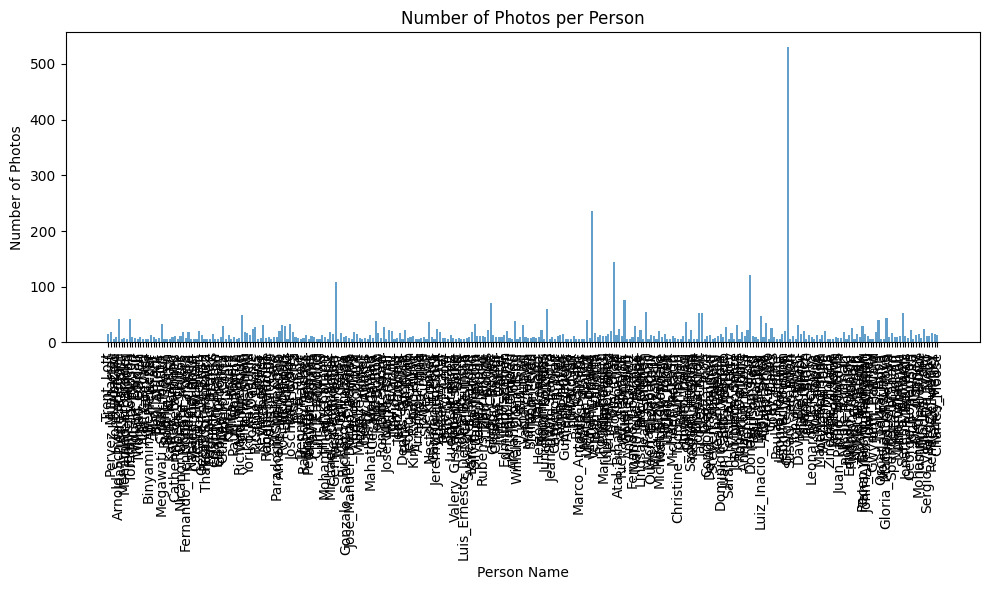
\includegraphics[width=0.75\linewidth]{WhatsApp Image 2024-04-21 at 14.23.53_a72961c7.jpg}
    \caption{No. of photos per unique identity}
    \label{fig:enter-label}
\end{figure}

\vspace{20pt}

In pre-processing the data,we picked out a few identites whose no. of images are greater than 70 each. Which are as follows-
\begin{figure}[H]
    \centering
    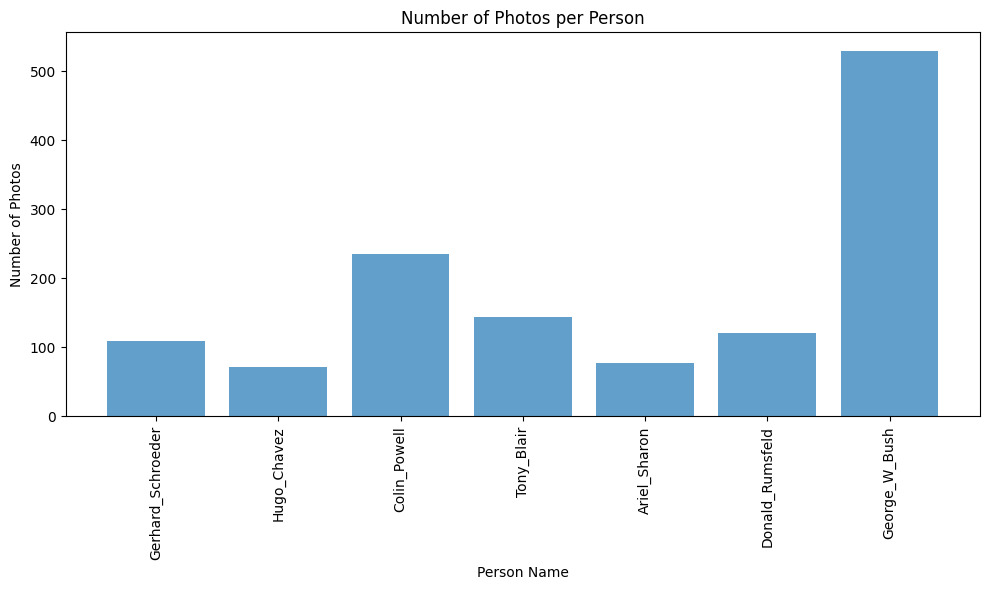
\includegraphics[width=1\linewidth]{WhatsApp Image 2024-04-21 at 14.23.53_b7e0dd4a.jpg}
    \caption{Unique identities with more than 70 images}
    \label{fig:enter-label}
\end{figure}

 Let's have a look at the results we obtained upon Local Binary pattern extraction-
 \begin{figure}[H]
     \centering
     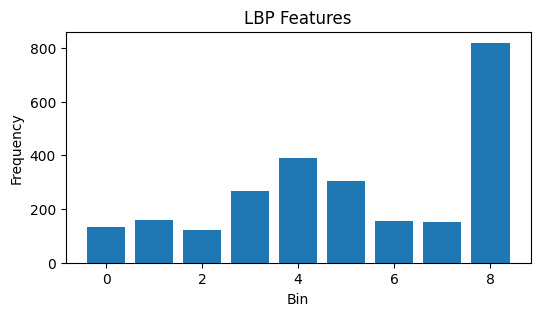
\includegraphics[width=1\linewidth]{WhatsApp Image 2024-04-21 at 14.23.53_79ad58bf.jpg}
     \caption{George Bush's case}
     \label{fig:enter-label}
 \end{figure}
 \begin{figure}[H]
     \centering
     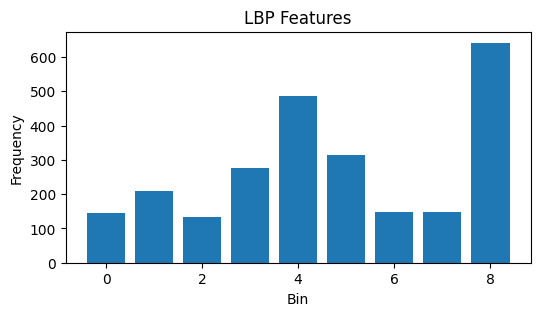
\includegraphics[width=1\linewidth]{WhatsApp Image 2024-04-21 at 14.24.04_e4267b1a.jpg}
     \caption{Tony Blair's case}
     \label{fig:enter-label}
 \end{figure}

 Then, we move on to CNN feature extraction and see analogous results-
 \begin{figure}[H]
     \centering
     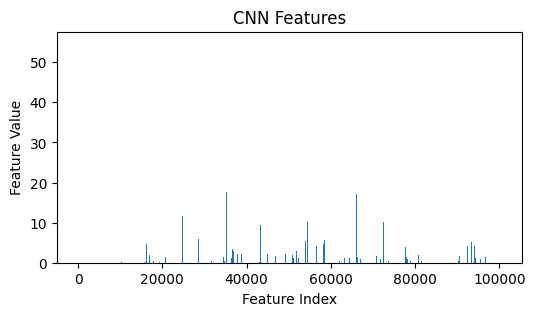
\includegraphics[width=1\linewidth]{WhatsApp Image 2024-04-21 at 14.23.53_f8ac10e0.jpg}
     \caption{George Bush's case }
\begin{figure}[H]
         \centering
         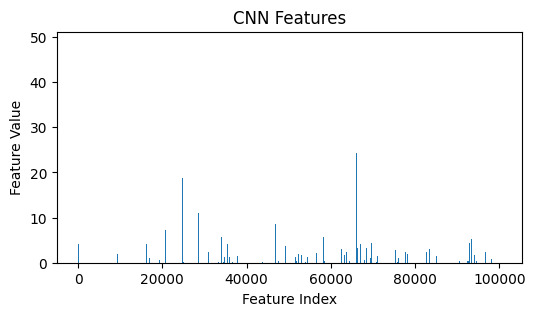
\includegraphics[width=1\linewidth]{WhatsApp Image 2024-04-21 at 14.24.04_a447d26f.jpg}
         \caption{Tony Blair's case}
         \label{fig:enter-label}
     \end{figure}
          \label{fig:enter-label}
 \end{figure}
 Similarly, we have a look at the HoG Results of these two concerned identities-
 \begin{figure}[H]
     \centering
     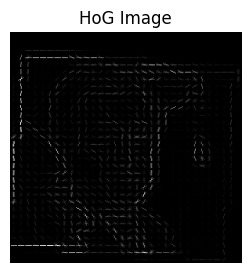
\includegraphics[width=0.5\linewidth]{WhatsApp Image 2024-04-21 at 14.27.12_e2561c98.jpg}
     \caption{George Bush HoG}
\begin{figure}[H]
         \centering
         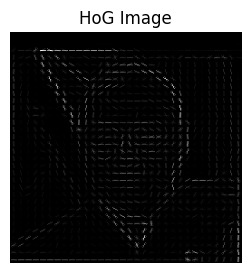
\includegraphics[width=0.5\linewidth]{WhatsApp Image 2024-04-21 at 14.27.33_57021518.jpg}
         \caption{Tony Blair HoG }
         \label{fig:enter-label}
     \end{figure}
          \label{fig:enter-label}
 \end{figure}

 Lastly, we obatined these results as far as no. of components are concerned with respect to Principal Component Analysis-
 \begin{figure}[H]
     \centering
     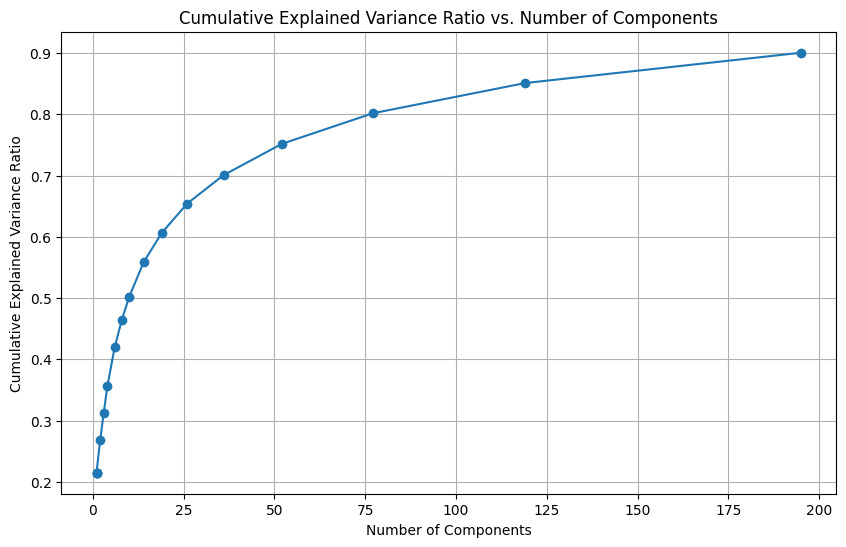
\includegraphics[width=0.75\linewidth]{WhatsApp Image 2024-04-21 at 14.24.12_4f165bf8.jpg}
 \end{figure}
 \section{Summary}
	\label{sec:app}
	We began with pre-processing the dataset where primarily we removed those unique identities with less than 70 corresponding images each. Then we did a standard 80:20 Train-test split on the dataset that remained. 
 \newline
 Once this is done,we employed several methods where principally we implemented them and then tested their accuracies with the help of different classifiers like SVM,KNN,Logistics regresssion,Random Forest,Gradient booster etc. At the core of it,lies formally feature extraction using the methods aforementioned like LDA,PCA,CNN,HOG etc. 
 \newline 
 Of all these processes we tried,we found out that our approach that of LDA with SVM Classifier alongwith RBF kernel attained\textbf{ highest test accuracy of 88.6 percentage}. The rest of the lesser fruitful results are mentioned below.
 \begin{figure}[h]
     \centering
     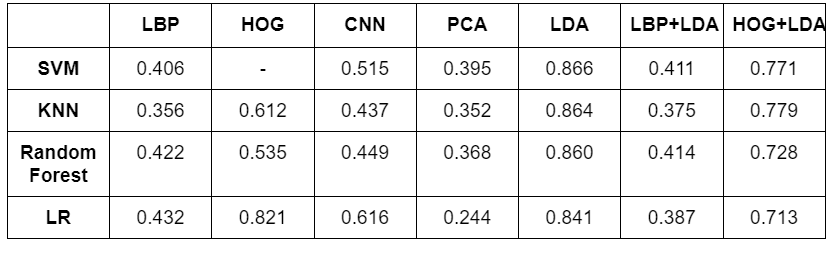
\includegraphics[width=1\linewidth]{image.png}
   
     \label{fig:enter-label}
 \end{figure}
 \newline
 Since this approached proved to be the most successful,we implemented that on our demo webpage of the project ultimately for random testing and demonstration purposes. 
 

\section{ References and Bibliography}
\begin{enumerate}
    \item \href{https://www.kaggle.com/datasets/jessicali9530/lfw-dataset}{\underline {\color{blue}LFW Dataset}}
    \item \href{https://towardsdatascience.com/hog-histogram-of-oriented-gradients-67ecd887675f}{\color{blue}https://towardsdatascience.com/hog-histogram-of-oriented-gradients-67ecd887675f}
    \item \href{https://ieeexplore.ieee.org/document/9012507}{\color{blue}https://ieeexplore.ieee.org/document/9012507}
    \item \href{https://www.youtube.com/watch?v=UbCWoMf80PY}{\color{blue}https://www.youtube.com/watch?v=UbCWoMf80PY}
\end{enumerate}


\section{Important Links }
\begin{enumerate}
    \item GitHub Repository: \href{https://github.com/dhyeyinf/Face_Identification}{\textbf{\underline {\color{blue}GitHub}}}
    \item Web Demo: \href{http://172.31.8.157:5000/}{\textbf{\textit{\underline {\color{blue}Click here}}}}
    \item YouTube demo video: \color{blue} \href{https://youtu.be/rYlWvNh9VCs}{\underline {\textbf{Demo Video}}}



\end{enumerate}
	

	
	\bibliography{refs}
	
	\appendix 
 \vfill
	
	\section{Contribution of each member}
	\label{sec:contribution}
	\begin{enumerate}
	\item Dhyey Findoriya (B22EE024) : Developed PCA feature extraction codebase,dataset exploration and pre-processing,prepared mid-term report.
	\item Akshat Patidar (B22EE087) : Developed HOG Codebase,applied LDA on HoG and CNN too. Also led backend of the webpage.
 \item 	 Manas Chechani (B22AI053) : Primarily constructed the webpage and working web-demo of the project. Contributed to the codebase of LDA and helped in the Pre-Processing of dataset.
 \item Nisarg Vaghela (B22EE068): Primarily led report preparation. Worked on codebase of LBP. Helped in preparing and editing the video demonstration.
 \item Ankit Raj (B22CS010):  Helped in Report preparation,contributed in CNN model codebase.
	
	\end{enumerate}
    	
\end{document}
